%----------------------------------------------------------------------------------------
%	SLIDE 8.
%----------------------------------------------------------------------------------------
\begin{frame}
\frametitle{Race condition}
\framesubtitle{A simple (but kinda dumb) example}

\begin{columns}
	\column{0.5\linewidth}
	\begin{figure}
		{\centering\small\textit{race-condition-serial.cpp}}
		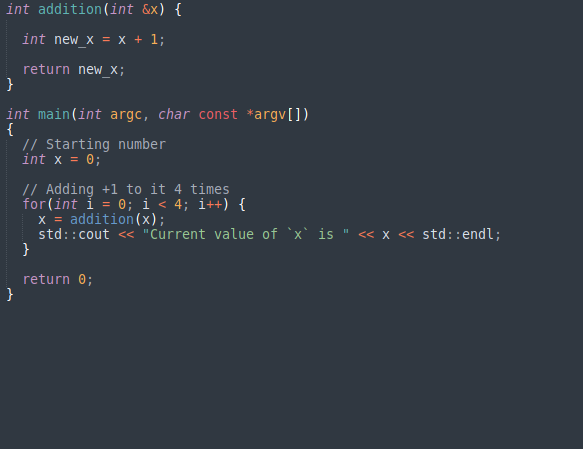
\includegraphics[width=\textwidth]{img/race-cond-ser.png}	
	\end{figure}
	\vspace*{-15pt}
	\begin{figure}
		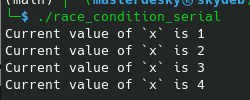
\includegraphics[width=0.7\textwidth]{img/race-cond-ser-output.png}
	\end{figure}
	
	\column{0.5\linewidth}
	\begin{figure}
		{\centering\small\textit{race-condition-parallel.cpp}}
		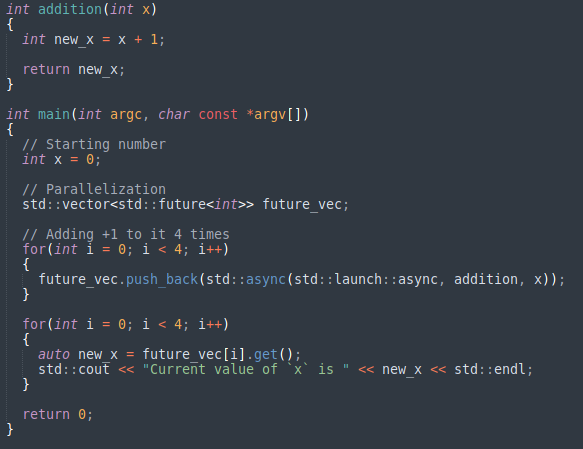
\includegraphics[width=\textwidth]{img/race-cond-par.png}
	\end{figure}
	\vspace*{-15pt}
	\begin{figure}
		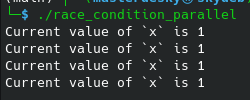
\includegraphics[width=0.7\textwidth]{img/race-cond-par-output.png}
	\end{figure}
	
\end{columns}

\end{frame}